%\newpage
\section{Wiederholung des Signifikanztests nach Entfernung der Extrema}
\label{Add:Pruemper:neuer_ttest:frage_2_und_3}

\begin{table}[H]
    \centering
    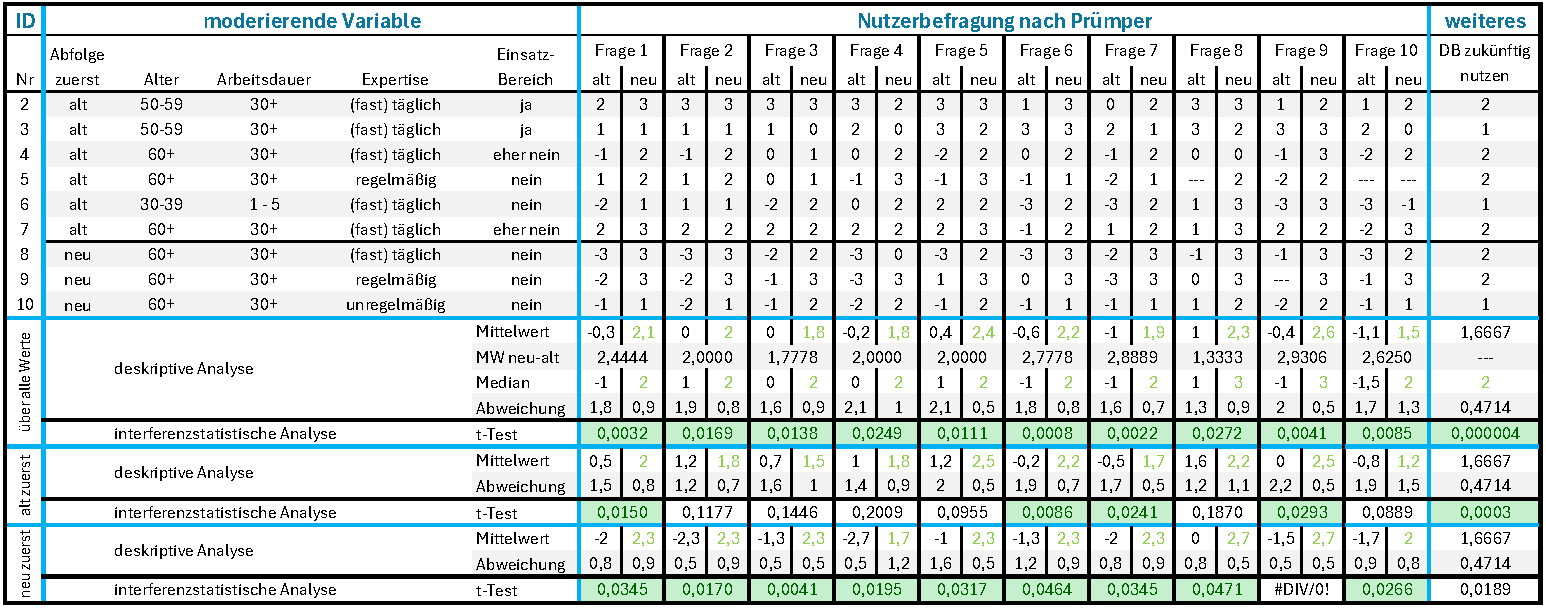
\includegraphics[width=0.8\textheight, angle=90]{Anhänge/05_Nutzerbefragung/Bilder/rohe_Daten_ohne_Extrema.pdf}
    \caption{Ergebnisse der Nutzerbefragung nach Prümper nach Entfernung der Extrema - Tabellarische Daten (Ausschnitt aus \autoref{tab:Nutzerbefragung:rohe_Daten})}
    \label{tab:Nutzerbefragung:rohe_Daten:ohne_Extrema_2_und_3}
\end{table}

\begin{figure}[H]
    \centering
    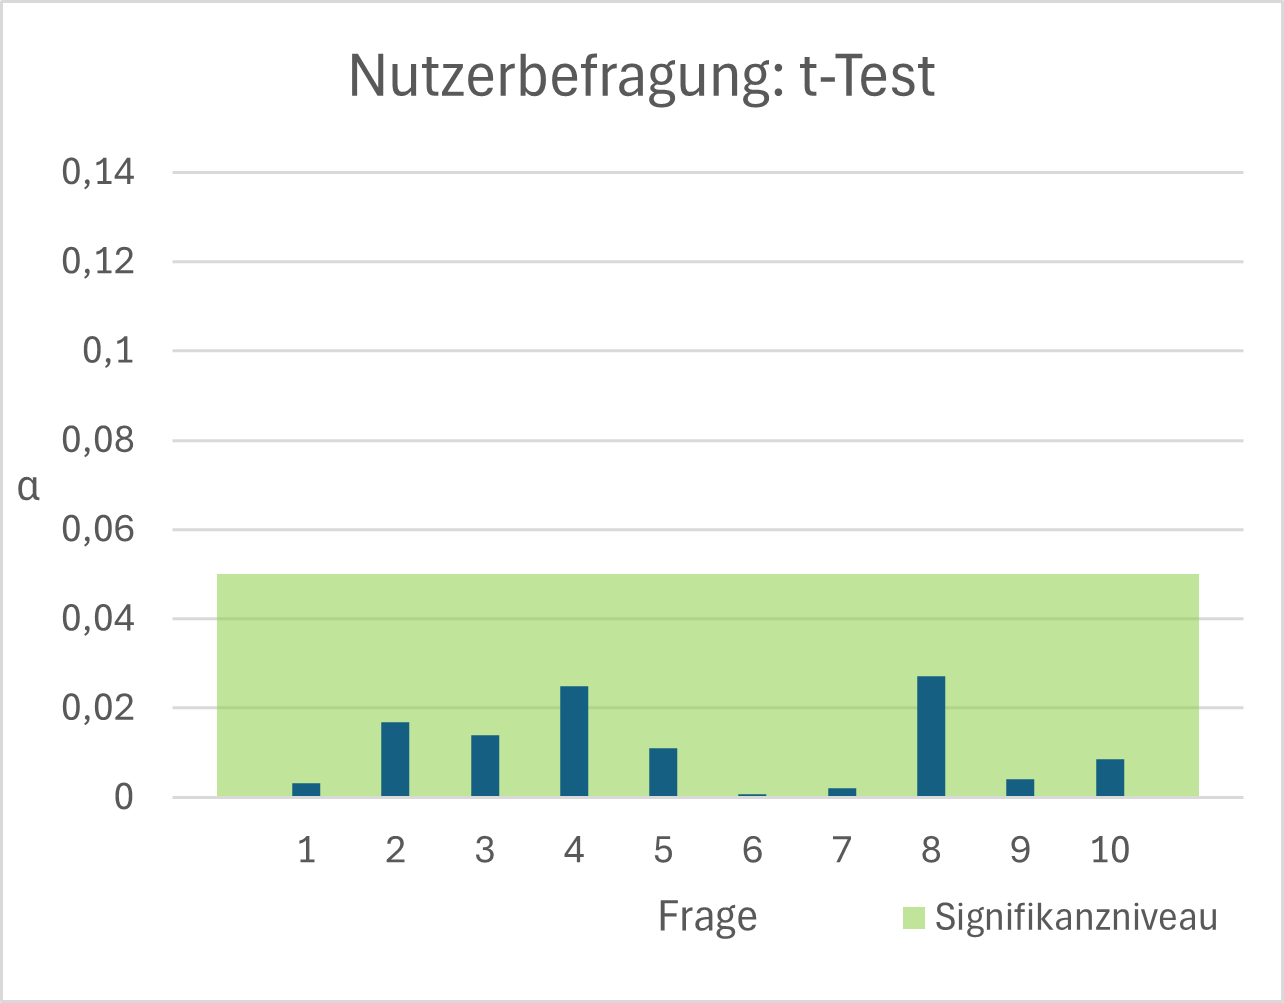
\includegraphics[width=0.8\linewidth]{Anhänge/05_Nutzerbefragung/Bilder/Signifikanzniveau_ohne_Extrema.png}
    \caption{Ergebnisse der Nutzerbefragung nach Entfernung der Extrema - t-Test-Ergebnisse (Daten aus \autoref{tab:Nutzerbefragung:rohe_Daten:ohne_Extrema_2_und_3})}
    \label{fig:Nutzerbefragung:ttest+Signifikanzniveau:ohne_Extrema_2_und_3}
\end{figure}